\section{Jackson und das Jackson Projekt}
Das Jackson Projekt entwickelt eine freie und modulare Bibliothek f\"ur die Serialisierung und Deserialisierung von Java-Instanzen in \ac{JSON}-Dokumente. Jackson wird unter der Contributor License Agreement (CLA) vermarktet. Die zur Zeit aktuelle Version ist 2.4.1, welche auch bei der Bearbeitung des Projektes eingesetzt wird.

\subsection{Jackson-Module}
Die Jackson-Bibliothek besteht aus drei Hauptmodulen, welche wie folgt bezeichnet sind:
\begin{itemize}
 \item "`jackson-core"' welches die JSON spezifische Implementierung sowie eine low-level streaming API enth\"alt
 \item "`jackson-annotations"' welches die Jackson spezifischen Annotationen enth\"alt.
 \item "`jackson-databind"' welches f\"ur das \textit{databind} verantwortlich ist.
\end{itemize}
Unter Databind wird eine Methode verstanden, welche \"uber ein User-Interface gesteuert werden kann.
Diese Methode ist in der Lage Daten aus einem Datenstrom wie zum Beispiel einem JSON-File zu lesen oder zu schreiben.

Mit diesen drei Modulen ist Jackson voll einsetzbar und kann Java-Instanzen zu einem JSON-Datenstrom umwandeln. Der JSON-Datenstrom wiederum kann gespeichert oder an andere Programme gesendet werden.

Um jedoch einheitliche Annotationen f\"ur Jackson und JAXB zu haben, wird ein weiteres Jackson-Modul ben\"otigt, welches in der Lage ist die JAXB-Annotationen zu verarbeiten.\cite{Jackson}

\subsection{Serialisierung mit Jackson}\label{Serialisierung}
Um eine Serialisierung mit Jackson umzusetzen wird zuerst eine Instanz der Klasse \texttt{ObjectMapper} ben\"otigt, welche den Databinder darstellt. Der \texttt{mapper} ist somit f\"ur die Convertierung von Java-Instanzen zu JSON-Dokumenten verantwortlich. 

Jedoch wird nicht nur der "`Converter"' ben\"otigt, sondern auch ein \texttt{AnnotationInspector}. Der \texttt{inspector} wird als Instanz von \texttt{JaxbAnnotationInspector} erstellt, welchem eine \texttt{TypeFactory} mit "`Default-Einstellungen"' \"ubergeben wird. Dies bedeutet es wird auf die Original JAXB-Annotationen geparst, ohne auf Sonderf\"alle zu achten. Andere Annotation werden nicht ber\"ucksichtigt. Der \texttt{inspector} wird nun dem "`Converter"' \"ubergeben, damit dieser auf die entsprechnden Annotationen reagieren kann.

Um eine \textit{Minimale Exception Safety} zu garantieren wird nun eine \texttt{Null}-Abfrage des zu serialisierenden Elements gemacht. Mit dieser Stufe der Sicherheit soll nicht verhindert werden das eine Exception passiert. Es wird lediglich garantiert das die Methode ohne Abzust\"urzen durchlaufen werden kann. \cite{ExceptionSafety}

Ist die zu serialisierende Instanz \texttt{Null} so wird eine \texttt{IllegalagumentException} generiert und die Methode so ordnungsgem\"a\ss{} beendet. Ist eine Instanz vorhanden, wird diese dem \texttt{mapper} \"ubergeben. Das Ergebnis des Aufrufs von \texttt{writeValueAsString} ist entweder bei Erfolg ein valider JSON-String oder beim scheitern eine \texttt{JsonProcessingException}.

Dieser Zusammenhang ist noch einmal im folgenden Quellcode-Beispiel beschrieben.
\newpage
\lstinputlisting{Code/Jackson_bsp.java}

\subsection{Deserialisierung mit Jackson}
F\"ur die Deserialisierung mit Hilfe von Jackson wird wie bei der Serialisierung ebenfalls ein Databinder und AnnotationInspector ben\"otigt, welche wie im Kapitel \ref{Serialisierung} erstellt werden. 

Bevor dies jedoch passiert, wird gepr\"uft ob der eingegebene String weder \texttt{Null} noch \texttt{Empty} ist. 
Sollte das der Fall sein, wird die Methode \texttt{readValue} mit dem \"ubergebenden String und der Information um welche Klassen-Instanz es sich beim String handelt \"ubergeben.

Die Schwierigkeit beim Deserialisieren besteht also nun darin, das bevor der String \"uberhaupt deserialisiert werden kann erst festgestellt werden muss um welche Klasse es sich eigentlich handelt.

Im Codebeispiel unten wird momentan noch davon ausgegangen, das es sich immer um eine Instanz der Klasse "`TestData"' handelt. Wie diese Einsch\"ankung aufgehoben werden kann wird im folgenden Kapitel beschrieben.

\lstinputlisting{Code/Jackson_des_bsp.java}
\subsection{Klassendiagramm der Serialisierung}

Wie von OPM verlangt erben hier alle Klassen von OPMObject. Um diese Arbeit mit der von Herrn Achim Walz vergleichen zu k\"onnen wurde sich auf eine gemeinsame abstrakte Klasse \texttt{Serializer} geeinigt. 

Die Klasse \texttt{JSONSerializer} erbt um einen Direkten vergleichen durchf\"uhren zu k\"onnen genau wie \texttt{XMLSerializer} von \texttt{Serializer}.
\texttt{Testdata} und \texttt{TestData2OPM} sind erste Test-Klassen von denen Instanzen serialisiert und deserialisiert werden.

Main-Klasse in diesem Projekt ist \texttt{OPM\_Serializer}. Die \texttt{main}-Methode setzt die Serialisierung im Test in Gang.

Damit wie gew\"unscht jede Klasse serialisiert werden kann, wurde die Methode \texttt{serializeMe} zu OPMObject hinzugef\"ugt.
Diese Methode nutzt nun bei Aufruf die \texttt{serialize}-Methode des jeweiligen Serialisierers.

Ein vollst\"andiger \"Uberblick ist im Klassendiagramm unten zu finden gegeben.


\FloatBarrier
\begin{figure}[ht]
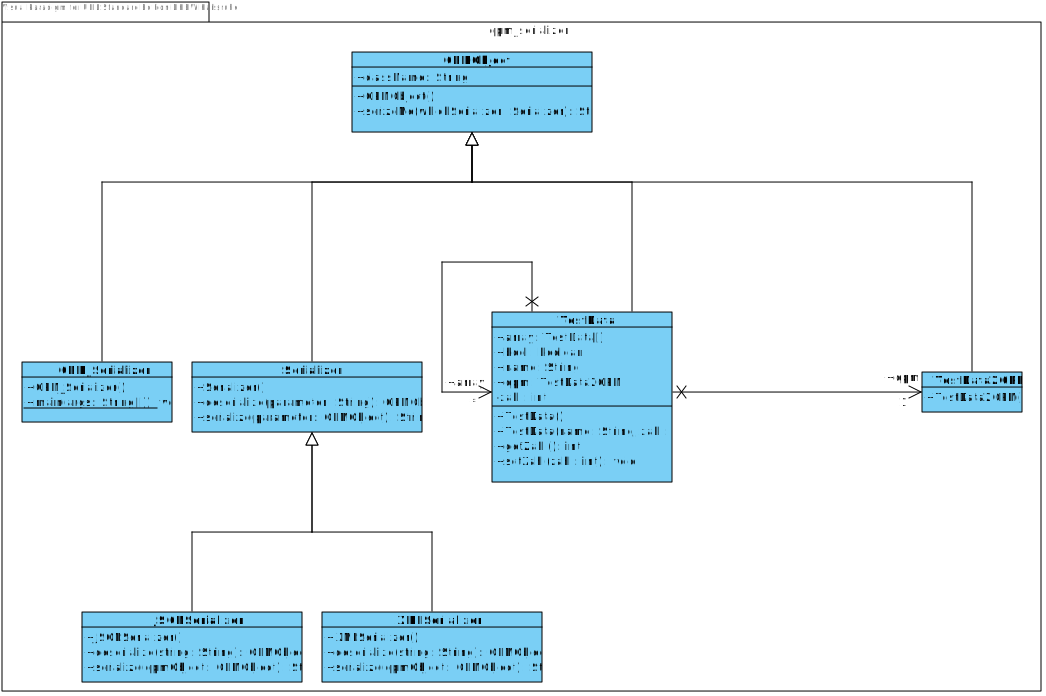
\includegraphics[width=16cm]{Bilder/Erstes_EKD}
\label{Klassendiagramm der Serialisierung}
\caption{Klassendiagramm der Serialisierung} 
\end{figure}




